\chapter{Dinâmica da partícula}
\label{Chap:Dinâmica}
%%%%%%%%%%%%%%%%%%%%%%%%%%%%%%%%%%%%%%%%%
%\minitoc

%\clearpage

%%%%%%%%%%%%%%%%%%%%%%%%%%%%%%%%%%%%%%%%%
\section{Introdução}
{\it

Para descrever o movimento de um corpo, precisamos de um referencial. O movimento é então descrito a partir de vetores que partem da origem do sistema de referência e terminam na posição do corpo. Outra característica interessante do movimento, é a velocidade com que ele ocorre. Ambas estão ligadas a situações práticas do tipo ``tenho \np[min]{15} para chegar à sala de aula antes que a aula comece.'': você ocupa uma posição, deseja ir para outra e tem um certo tempo para realizar tal deslocamento.

Também descrevemos a aceleração, que é a ``taxa de variação da velocidade por unidade de tempo'', ou seja, quanto a velocidade muda em uma unidade de tempo. Dentro da cinemática, tal grandeza se limitou -- ao menos no nosso estudo -- a ser uma constante. Entretanto, em uma freada brusca de um ônibus, situação onde temos uma grande desaceleração, observamos a atuação de forças muito intensas. Se estivermos em pé dentro do ônibus, precisamos fazer um grande esforço para não cair, segurando-se aos apoios afixados ao teto ou aos bancos. Em uma freada mais moderada, o esforço já não é tão grande. Vemos, através disso, que a força e a aceleração estão ligadas de alguma maneira. Vamos então tratar do problema da \emph{dinâmica}, nos preocupando com as causas do movimento.
}

\comment{sumário do que conseguimos com cinemática, enfatizar a questão de referencial, objetivos da dinâmica}

%%%%%%%%%%%%%%%%%%%%%%%%%%%%%%%%%%%%
\section{Conceitos de força e massa}
%%%%%%%%%%%%%%%%%%%%%%%%%%%%%%%%%%%%

Não adianta, precisamos discutir isso antes de qq coisa. Falar sobre força com noções de senso comum, mas argumentar que dois objetos podem ou não estar exercendo força um sobre o outro quando em contato (imagine dois blocos, um sobre o outro, ou um ao lado do outro, sobre uma mesa). 



An impress'd force is an action exerted upon a body, in order to change its state, either of rest, or of moving uniformly forward in a right line.
This force consists in the action only; and remains no longer in the body, when the action is over. For a body maintains every new state it acquires, by its Vis Inertiæ only. Impress'd forces are of different origines; as from percussion, from pressure, from centripetal force. 

ao falar de massa, tomar a definição de Newton tb:


The Quantity of Matter is the measure of the same, arising from its density and bulk conjunctly.

Principia - 1729 - Definitions - Illuminated T.pngHUS AIR of a double density, in a double space, is quadruple in quantity; in a triple space, sextuple in quantity. The same thing is to be understood of snow, and fine dust or powders, that are condensed by compression or liquefaction; and of all bodies that are by any causes whatever differently condensed. I have no regard in this place to a medium, if any such there is, that freely pervades the interstices between the parts of bodies. It is this quantity that I mean hereafter everywhere under the name of Body or Mass. And the same is known by the weight of each body, for it is proportional to the weight, as I have found by experiments on pendulums, very accurately made, which shall be shewn hereafter.


%%%%%%%%%%%%%%%%%%%%%%%%%%%%%%%%%%%%%%%%%%%%%%%%%%%%%%%%%%%%%%%
\section{Princípio da Inércia segundo Galileu e segundo Newton}
%%%%%%%%%%%%%%%%%%%%%%%%%%%%%%%%%%%%%%%%%%%%%%%%%%%%%%%%%%%%%%%

Segundo a física aristotélica, para que haja movimento, existe a necessidade de que uma força atue sobre um objeto. Assim, para que um bloco se mantenha em movimento, é necessário que sobre ele haja uma força. Aparentemente esta observação descreve razoavelmente um experimento cotidiano, afinal, se empurramos uma caixa sobre um piso, ela certamente para após cessarmos a força aplicada sobre ela. Ao atirarmos um objeto -- como uma flecha ou uma pedra -- no entanto, observamos algo diferente: cessamos a interação com o objeto, cessando a força sobre ele aplicada, porém o movimento não cessa.

\comment{Colocar o texto aqui, como no Moysés, depois enumerar as observações importantes}
Galileu analisou o movimento de esferas que podem subir ou descer rampas, tecendo as seguintes observações:
\begin{itemize}
  \item Se tomarmos uma superfície inclinada lisa e resistente, juntamente com uma esfera também lisa e resistente. Colocamos segunda sobre a primeira, de forma que fique livre para rolar tomando cuidado para remover todos os possíveis ``impedimentos'' ao movimento. Desprezamos também a resistência do ar. Observamos que a esfera rola em direção à parte mais baixa da superfície, ganhando velocidade continuamente enquanto dura a descida. Quanto maior a inclinação do plano em relação à horizontal, maior é o ganho de velocidade da esfera após percorrer uma dada distância.
  \item Para que a esfera suba o plano, é necessário que ela seja atirada com velocidade, ou arrastada, plano acima. Sendo atirada, o seu movimento natural é perder velocidade continuamente, eventualmente parando. Se aumentamos ou diminuímos a inclinação do plano, mantendo constante a velocidade com que a esfera foi atirada, temos que ela percorrerá uma distância maior ou menor, sendo tanto maior quanto menor for a inclinação e vice-versa.
  \item Se tomarmos uma superfície perfeitamente horizontal, não existe tendência a ganhos de velocidade, nem de perdas de velocidade. Se colocarmos a esfera de forma que ela fique parada sobre a superfície, ela deve permanecer parada. Se a colocarmos em movimento, não havendo impedimentos, ela deve permanecer em movimento. Não havendo inclinação do plano, não há razão para haver aumento ou diminuição da velocidade. Se o plano horizontal for infinito, ela deve continuar nesse movimento indefinidamente. A razão disto é que existe uma tendência dos corpos a se moverem em direção ao centro da Terra. Como em um plano horizontal todas as partes estão à mesma distância em relação ao centro, não existe um lugar preferencial da superfície para o qual a esfera tem uma tendência a se dirigir. Tal superfície seria, na realidade, uma esfera lisa e concêntrica com a Terra. Uma vez posta em movimento em direção ao norte, por exemplo, a esfera continuaria a se mover em tal direção até atingi-lo e passar a se mover para o sul, descrevendo um circulo em torno da Terra.
\end{itemize}
%
Resumindo, podemos afirmar que -- segundo Galileu -- \emph{um corpo sobre uma superfície horizontal continuará se movendo na mesma direção com velocidade constante a não ser que seja perturbado}. Portanto, pela primeira vez se vislumbra o princípio da inércia. Devemos destacar que para Galileu, \emph{o movimento horizontal do corpo não é retilíneo}, mas um círculo em torno da Terra -- essa é a interpretação mais comum das principais obras de Galileu, porém há controvérsias sobre isso: veja \cite{Vasconcelos2005} --. Finalmente, através de tais observações, Galileu concluiu que é impossível distinguir um corpo em movimento com velocidade constante de outro parado, a não ser que tenhamos uma referência externa.

Em seu livro, \emph{Principia}, Newton declara a primeira lei do movimento como
\begin{quote}
  Todo corpo permanece em estado de repouso, ou de movimento uniforme em uma linha reta, a não ser que seja compelido a mudar tal estado por forças que atuam sobre ele.
\end{quote}
%
A diferença fundamental em relação ao proposto por Galileu é o fato de que o movimento, na ausência de forças, se dá em \emph{linha reta}. Verificamos no Capítulo ?? que se temos uma mudança na direção da velocidade, temos uma aceleração, mesmo que o módulo desse vetor se mantenha constante. Veremos através da Segunda Lei de Newton, a seguir, que se não temos força, não temos aceleração. Consequentemente, na ausência de forças atuando sobre um corpo que se desloca, o movimento deve ser retilíneo e com o módulo da velocidade constante.

%%%%%%%%%%%%%%%%%%%%%%%%%%%%%%%%%%%%
%\subsection{Referenciais inerciais}
%%%%%%%%%%%%%%%%%%%%%%%%%%%%%%%%%%%%

% %%%%%%%%%%%%%%%%%%%%%%%%%%%%%%%%%%%%
% \subsection{Origem do termo inércia} % wikipedia
% %%%%%%%%%%%%%%%%%%%%%%%%%%%%%%%%%%%%
% 
% sobre a inércia:
% The vis insita, or innate force of matter, is a power of resisting, by which every body, as much as in it lies, endeavours to persevere in its present state, whether it be of rest, or of moving uniformly forward in a right line.
% 
% This force is ever proportional to the body whose force it is; and differs nothing from the inactivity of the mass, but in our manner of conceiving it. A body, from the inactivity of matter, is not without difficulty put out of its state of rest or motion. Upon which account, this vis insita, may, by a most significant name, be called vis inertiæ, or force of inactivity. But a body exerts this force only, when another force, impressed upon it, endeavours to change its condition; and the exercise of this force may be considered both as resistance and impulse; it is resistance, in so far as the body, for maintaining its present state, withstands the force impressed; it is impulse, in so far as the body, by not easily giving way to the impressed force of another, endeavours to change the state of that other. Resistance is usually ascribed to bodies at rest, and impulse to those in motion; but motion and rest, as commonly conceived, are only relatively distinguished; nor are those bodies always truly at rest, which commonly are taken to be so.
% 
% The actual term "inertia" was first introduced by Johannes Kepler in his Epitome Astronomiae Copernicanae (published in three parts from 1618–1621); however, the meaning of Kepler's term (which he derived from the Latin word for "idleness" or "laziness") was not quite the same as its modern interpretation. Kepler defined inertia only in terms of a resistance to movement, once again based on the presumption that rest was a natural state which did not need explanation. It was not until the later work of Galileo and Newton unified rest and motion in one principle that the term "inertia" could be applied to these concepts as it is today.[citation needed]
% 
% Nevertheless, despite defining the concept so elegantly in his laws of motion, even Newton did not actually use the term "inertia" to refer to his First Law. In fact, Newton originally viewed the phenomenon he described in his First Law of Motion as being caused by "innate forces" inherent in matter, which resisted any acceleration. Given this perspective, and borrowing from Kepler, Newton actually attributed the term "inertia" to mean "the innate force possessed by an object which resists changes in motion"; thus Newton defined "inertia" to mean the cause of the phenomenon, rather than the phenomenon itself. However, Newton's original ideas of "innate resistive force" were ultimately problematic for a variety of reasons, and thus most physicists no longer think in these terms. As no alternate mechanism has been readily accepted, and it is now generally accepted that there may not be one which we can know, the term "inertia" has come to mean simply the phenomenon itself, rather than any inherent mechanism. Thus, ultimately, "inertia" in modern classical physics has come to be a name for the same phenomenon described by Newton's First Law of Motion, and the two concepts are now considered to be equivalent.
% 
%%%%%%%%%%%%%%%%%%%%%%%%%%%%%%%%%%%%%%%%%%%%%%%
\section{Segunda Lei de Newton}
%%%%%%%%%%%%%%%%%%%%%%%%%%%%%%%%%%%%%%%%%%%%%%%
%%%%%%%%%%%%%%%%%%%%%%%%%%%%%%%%%%%%%%%%%%%%%%%
\subsection{Relação entre força e aceleração}
%%%%%%%%%%%%%%%%%%%%%%%%%%%%%%%%%%%%%%%%%%%%%%%

Através da Lei da Inércia, damos um passo adiante no estudo do movimento dos corpos, associando força a aceleração. Segundo Newton
\begin{quote}
  A alteração do movimento é sempre proporcional à força motriz a ele aplicada; e é feita na direção da linha reta em que tal força atua.\footnote{Newton usa o termo \emph{movimento} para o que conhecemos hoje como \emph{quantidade de movimento} ou \emph{momento linear}, representado por $p$. Tal definição, dada por $p = mv$ engloba tanto a massa quanto a velocidade, sendo que sua alteração pode se dar por meio de uma \emph{variação} da massa ou da velocidade, ou seja, sua alteração se dá através da aceleração, se $m$ for mantido constante.}
\end{quote}
%

Experimentalmente, podemos verificar que a aceleração de um objeto é maior caso a força que exercemos sobre ele seja maior. Se temos uma alteração da velocidade quando um corpo se desloca por certo tempo sob ação de uma força, ao dobrarmos ou triplicarmos a intensidade da força, teremos que a alteração da velocidade dobrará ou triplicará, respectivamente. Podemos então dizer que
\comment{falar sobre características vetoriais da força e já escrever essa relação vetorialmente}
\begin{equation}
  a \propto F.
\end{equation}

\begin{marginfigure}[1cm]
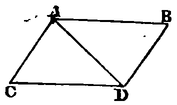
\includegraphics{Fig/177px-Principia1846-084.png}
\caption{Figura utilizada por Newton para explicar a composição da ação das forças.}
\end{marginfigure}

\comment{Quote do texto deo Newton, mostrar que as distâncias estão relacionadas às acelerações. Mostrar modernamente com vetores. Figure vetorial com aceleração e deslocamento.}
Newton ainda considera a possibilidade de que das forças atuem sobre um corpo ao mesmo tempo. Nesse caso, se considerarmos a atuação de uma só força, o corpo se deslocará, em um dado tempo, uma certa distância na direção da força. Analogamente, quando a outra atua sozinha sobre o corpo, temos um deslocamento na direção da segunda, ainda considerando o mesmo intervalo de tempo. Se ambas as forças atuarem sobre o corpo, no mesmo intervalo de tempo, o deslocamento resultante será dado pela reta que forma a diagonal do paralelogramo formado pelos dois deslocamentos individuais. De uma maneira mais direta, podemos dizer que a aceleração sofrida pelo corpo é dada pela soma vetorial das acelerações individuais que as forças -- agindo sozinhas, uma de cada vez -- imprimem sobre o corpo. O que, por sua vez, define uma força resultante que é dada pela soma das duas forças.

\comment{concluir alguma coisa a partir do parágrafo, se possível (que essas são as propriedades de um vetor); Temos que falar sobre força resultante tb. e discutir que é ela que determina a aceleração (fácil se pensarmos em um bloco submetido a duas forças, por exemplo)}

%%%%%%%%%%%%%%%%%%%%%%%%%%%%%%%%%%%%%%%%%%%%%
\subsection{Relação entre massa e aceleração}
%%%%%%%%%%%%%%%%%%%%%%%%%%%%%%%%%%%%%%%%%%%%%

Newton define a noção de \emph{quantidade de matéria}, ou \emph{massa}:
\begin{quote}
\emph{A quantidade de matéria é uma medida da mesma, advindo de sua densidade e volume conjuntamente.}
  
Portanto, ar com o dobro da densidade, no dobro do volume, é o quadruplo em quantidade\footnote{A densidade é uma variável intensiva, enquanto o volume é uma variável extensiva. A segunda pode ser somada ao juntarmos dois sistemas, a primeira não.}; no triplo do volume, o sêxtuplo em quantidade. O mesmo se deve entender de neve, e poeira fina ou pós, que seja condensados por compressão ou liquefação; e de todos os corpos que sejam por qualquer motivo de alguma maneira condensados. [\dots]. É essa quantidade a que me refiro doravante [\dots] como corpo ou massa. E o mesmo é conhecido como peso de cada corpo; pois é proporcional ao peso, como descobri por experimentos em pêndulos, executados com muito cuidado, que serão mostrados adiante.
\end{quote}
%
Cabe aqui uma discussão acerca da confusão entre massa e peso. Como mostrado acima, Newton deixa claro que a massa é uma medida da quantidade de matéria que um corpo possui, estando associada tanto ao seu volume quanto à sua densidade, e que tal grandeza é \emph{proporcional} ao peso. Veja que o peso possui características vetoriais, pois é dirigido verticalmente para baixo e possui um módulo que é tão maior quanto maior forem sua densidade e seu volume -- isto é, quanto maior for sua quantidade de matéria, ou massa --. Além disso, como veremos adiante, um corpo que se encontra longe da superfície da Terra é atraído por uma força que varia com a distância de separação, sendo, portanto diferente para cada posição. A massa, por outro lado, é uma constante característica do corpo e não está sujeita a mudanças.

Se aplicarmos uma força resultante em um corpo, temos que ele estará sujeito a uma aceleração. No entanto, se aplicarmos uma dada força em um corpo muito massivo, teremos uma aceleração pequena, ao passo que se aplicarmos tal força em um corpo com uma massa pequena, teremos uma aceleração maior. Percebemos então que a aceleração assume uma proporcionalidade inversa em relação à massa:
\begin{equation}
  a \propto \frac{1}{m},
\end{equation}
%
ou, considerando a dependência em relação à força
\begin{equation}
  a \propto \frac{F}{m}.
\end{equation}
%
Considerando que a aceleração só dependa de $F$ e $m$, e também o fato de que uma proporcionalidade pode ser escrita como uma igualdade se utilizarmos uma constante de proporcionalidade $C$ qualquer -- cujo valor precisamos determinar -- temos
\begin{equation}
  a = C \frac{F}{m}.
\end{equation}

Apesar de termos unidades para a aceleração e para a massa, não temos para a força. Nesse caso, podemos englobar a constante $C$ na própria definição das unidades da força e obter
\begin{equation}
  a = \frac{F}{m},
\end{equation}
%
ou seja,
\begin{equation}
  F = m a. \mathnote{Segunda Lei de Newton.}
\end{equation}

%%%%%%%%%%%%%%%%%%%%%%%%%%%%%
\subsection{Medidas de massa}
%%%%%%%%%%%%%%%%%%%%%%%%%%%%%

Através da Segunda Lei de Newton, podemos determinar a massa de um objeto em relação à massa de outro. Suponha que tomamos um objeto qualquer e a ele aplicamos uma força resultante $F$. Sabemos que ele será submetido a uma aceleração de tal maneira que
\begin{equation}
  F = m_1 a_1.
\end{equation}
%
Se submetermos outro corpo à mesma força, temos
\begin{equation}
  F = m_2 a_2.
\end{equation}
%
Como a força é a mesma em ambos os casos, podemos escrever
\begin{equation}
  m_1 a_1 = m_2 a_2,
\end{equation}
%
ou
\begin{equation}
  m_2 = \frac{a_1}{a_2}m_1.
\end{equation}

Este resultado é relevante pois não temos um método de determinar a massa de um objeto a não ser por comparação com outro. No Sistema Internacional, utiliza-se a massa de um cilindro metálico como massa padrão em relação a qual as demais massas são medidas, sendo atribuída a ele a massa de \np[kg]{1}. Utilizando o processo acima, podemos determinar a massa de um objeto qualquer em relação ao padrão de referência.

%%%%%%%%%%%%%%%%%%%%%%%%%%%%%%%%
\section{Terceira Lei de Newton}
%%%%%%%%%%%%%%%%%%%%%%%%%%%%%%%%

A Terceira Lei de Newton foi por ele enunciada como
\begin{quote}
\emph{Para cada ação há sempre uma reação igual oposta: ou as ações mutuas de dois corpos um sobre o outro são sempre iguais, e dirigidas a partes contrárias.}

Qualquer coisa que puxa ou empurra outra é tão puxado ou pressionado quanto pela outra. Se você pressionar uma pedra com seu dedo, o dedo também é pressionado pela pedra. Se um cavalo puxa uma pedra amarrada a uma corda, o cavalo (se posso assim dizer) será igualmente puxado para trás em direção à pedra: pois a corda distendida, pelo mesmo esforço para relaxar ou se afrouxar, tanto puxará o cavalo em direção à pedra, quanto puxará a pedra em direção ao cavalo, e obstruirá o progresso de um tanto quanto avança aquele do outro. Se um corpo colide com outro, e por meio de sua força muda o movimento do segundo, o segundo corpo também (devido à igualdade da pressão mútua) sofrerá uma mudança igual, em seu próprio movimento, em direção à parte contrária. As mudanças feitas por essas ações são iguais, não nas velocidades, mas nos movimentos dos corpos; isto se os corpos não são obstados por outros impedimentos. Pois, devido ao fato de que os movimentos são igualmente alterados, as mudanças das velocidades efetuadas em direções a partes contrárias são reciprocamente proporcionais aos corpos [massas]. Esta lei também ocorre em atrações, como será provado adiante.
\end{quote}

Newton contempla a interação entre dois corpos quaisquer, seja por contato, seja à distância. Na interação um corpo exerce uma força sobre outro, porém sente os efeitos de uma força de mesmo módulo e direção, porém de sentido contrário. Se, por exemplo, um patinador arremessa uma bola com força, verificamos que a bola sofre uma grande alteração de sua velocidade. O patinador, por sua vez, sofre uma aceleração no sentido contrário -- no entanto, observamos que sua velocidade final é muito menor --. Isto pode ser entendido através da segunda lei de Newton, pois, como as forças que atuam são iguais em módulo
\begin{align}
  F &= m_1 a_1 \\
  F &= m_2 a_2
\end{align}
%
e, consequentemente,
\begin{equation}
  a_2 = \frac{m_1}{m_2} a_1.
\end{equation}
%
Logo, se supomos que a massa $m_1$ da bola é muito menor que a massa $m_2$ do patinador, temos que $m_1/m_2 \ll 1$ e -- consequentemente -- $a_2 \ll a_1$. Como ambos os corpos estão sujeitos às acelerações durante o mesmo intervalo de tempo, observamos que $v_2 \ll v_1$, pois a velocidade é diretamente proporcional à duração da aceleração.

Finalmente, é importante notar que o par ação-reação oriundo de uma interação nunca atua sobre o mesmo corpo. Devido ao fato de que uma força resulta da interação de dois corpos, não faz sentido supor que pudéssemos ter uma situação diferente. No caso de uma força interna, podemos recorrer à interpretação de que todos os corpos são constituídos de átomos, de onde verificamos que uma interação entre partes diferentes de um corpo são interações entre átomos (ou grupos de átomos, como moléculas) diferentes. Consequentemente, podemos afirmar que as forças de um par ação-reação, se dão entre corpos diferentes, mesmo no caso de forças internas.

%%%%%%%%%%%%%%%%%%%%%%%%%%%%%%%%%%%%%%%%%%%%%%%
\paragraph{Limitação da terceira lei de Newton}
%%%%%%%%%%%%%%%%%%%%%%%%%%%%%%%%%%%%%%%%%%%%%%%

Problema na força de Lorentz (ver Griffiths, Eletromagnetismo). Problema é resolvido se considerarmos a conservação do momento linear pois é possível se mostrar que há momento linear nos campos eletromagnéticos.

%%%%%%%%%%%%%%%%
\section{Forças}
%%%%%%%%%%%%%%%%

Através das Leis de Newton, fica evidente que transferimos o problema da determinação do movimento dos corpos para a determinação das forças que atuam sobre ele. Infelizmente, não existe uma lei que determine quais são as forças que atuam sobre um corpo, restando como única saída uma análise cuidadosa do fenômeno estudado.

A partir de experimentos, se tem o conhecimento de um pequeno número de forças que podem ser consideradas \emph{fundamentais}:
\begin{itemize}
  \item força gravitacional;
  \item força eletromagnética;
  \item força nuclear forte;
  \item força nuclear fraca.
\end{itemize}
%
Tais forças são denominadas fundamentais pois todas as demais podem ser interpretadas através delas. Em geral, no entanto, a descrição de fenômenos através delas não é prática. Do ponto de vista macroscópico, é mais útil trabalharmos com forças que surgem a partir de interações complexas dos átomos através das forças fundamentais. As duas primeiras são responsáveis pelas forças que estudaremos em mecânica, como a força peso (oriunda da força gravitacional) e as forças normal, de tensão, atrito, arrasto e elástica (oriundas da força eletromagnética). Outras expressões podem ser encontradas para outras situações, no entanto não as estudaremos a fundo aqui. Podemos citar como exemplo as forças que atuam sobre cargas elétricas, entre condutores portando corrente, entre moléculas (força de van der Waals), etc. Em alguns casos, vamos tratar de forças de contato que tem origem eletromagnética, porém que não nos damos ao trabalho de nomear, como as forças que atuam entre duas esferas que colidem.

%%%%%%%%%%%%%%%%%%%%%%%%%%%%%%
\paragraph{Diagramas de força} 
%%%%%%%%%%%%%%%%%%%%%%%%%%%%%%

\begin{marginfigure}
\centering
\begin{tikzpicture}[>=Stealth,
     interface/.style={
        % superfície
        postaction={draw,decorate,decoration={border,angle=-45,
                    amplitude=0.2cm,segment length=2mm}}},
    ]
    
    \draw[interface] (-1,0) -- (1,0);
    
    \draw[pattern= north west lines] (-0.5,0) rectangle (0.5,1);
    \draw[fill] (0,0.5) circle (1pt);
    
    \draw[->, thick] (0, 0.5) -- (0,-0.5) node[left]{$\vec{P}$};
    \draw[->, thick] (0,1) -- (0,2) node[left]{$\vec{N}$};
    
    \draw[fill] (2,0.5) circle (1pt);
    \draw[->, thick] (2,0.5) -- +(0,1) node[right]{$\vec{N}$};
    \draw[->, thick] (2,0.5) -- +(0,-1) node[right]{$\vec{P}$};
    
\end{tikzpicture}
\caption{Esboço de um problema e o diagrama de forças do problema. Apesar de a rigor devermos utilizar o diagrama, é mais ilustrativo utilizar a representação da esquerda, porém ela tem problemas conceituais: a força normal é exercida na parte inferior do bloco, não no topo, como ilustrado.}
\end{marginfigure}

falar de dividir a segunda lei em três eixos e utilizar o diagrama de força pra resolver problemas, falar da escolha do sistema de coordenadas: minimizar forças a serem decompostas, colocar a aceleração em um eixo só.

\begin{marginfigure}
\centering
\begin{tikzpicture}[>=Stealth, rotate=-35,
     interface/.style={
        % superfície
        postaction={draw,decorate,decoration={border,angle=-45,
                    amplitude=0.2cm,segment length=2mm}}},
    ]
   
    \draw[dashed, ->] (0,0.5) -- (4,0.5) node[below left]{$x$};
    \draw[dashed, ->] (2,-1) -- (2,2.2) node[below right]{$y$};
    
    \draw[interface] (0,0) -- (4,0);
    \draw[pattern= dots] (1.5,0) rectangle (2.5,1);
        
    \draw[fill] (2,0.5) circle (1pt);
    \draw[->, thick] (2,0.5) -- +(-55:1) node[left]{$\vec{P}$};
    \draw[->, thick] (2,1) -- +(0,0.81915) node[below right]{$\vec{N}$};
    
    \draw[->] (3,1) -- node[above]{$\vec{a}$}(3.7,1);
    
    \coordinate (A) at (4,0);
    \draw[dashed] (A) -- +(-145:1) coordinate (B);
    \coordinate (O) at (0,0);
    
    \draw[dashed] (A) -- (B);
    \pic [draw, "$\theta$", angle eccentricity=1.5] {angle = O--A--B};

\end{tikzpicture}
\caption{Escolhemos o sistema de coordenadas de maneira que a aceleração esteja contida em apenas um dos eixos.}
\end{marginfigure}


\begin{marginfigure}
\centering
\begin{tikzpicture}[>=Stealth, rotate=-35,
     interface/.style={
        % superfície
        postaction={draw,decorate,decoration={border,angle=-45,
                    amplitude=0.2cm,segment length=2mm}}},
    ]
     
    \draw[interface, gray] (0,0) -- (4,0);
    \draw[pattern= dots, pattern color = gray] (1.5,0) rectangle (2.5,1);
        
    \draw[fill, gray] (2,0.5) circle (1pt);
    \draw[->, thick, gray] (2,0.5) -- +(-55:1) node[left]{$\vec{P}$};
    \draw[->, thick, gray] (2,1) -- +(0,0.81915) node[below right]{$\vec{N}$};
       
    \path[name path = solo] (4,0)+(-145:3) -- +(35:1);
    \path[name path = eixop] (2,0.5) -- +(-55:1.75);
    \path[name path = eixox] (2,0.5) -- (5,0.5);
    \path[name path = eixoy] (2,0.5) -- +(0,-2);
    
    \draw[dashed, name intersections={of=solo and eixox}] (2,0.5) -- (intersection-1) coordinate (A);
    \draw[dashed, name intersections={of=solo and eixop}] (2,0.5) -- (intersection-1);
    \draw[dashed, name intersections={of=solo and eixoy}] (2,0.5) -- (intersection-1) coordinate (B);
    \draw[dashed] (A) -- (B);

    \coordinate (O) at (0,0.5);
    
    \pic [draw, "$\theta$", angle eccentricity=1.5] {angle = O--A--B};
    
    \coordinate (C) at (4,0);
    \coordinate (OS) at (0,0);
    \pic [draw, "$\theta$", angle eccentricity=1.5, gray] {angle = OS--C--B};
    
\end{tikzpicture}
\caption{Escolhemos o sistema de coordenadas de maneira que a aceleração esteja contida em apenas um dos eixos.}
\end{marginfigure}

\begin{marginfigure}
\centering
\begin{tikzpicture}[>=Stealth, rotate=-35,
     interface/.style={
        % superfície
        postaction={draw,decorate,decoration={border,angle=-45,
                    amplitude=0.2cm,segment length=2mm}}},
    ]
           
    \path[name path = solo] (4,0)+(-145:3) -- +(35:1);
    \path[name path = eixop] (2,0.5) -- +(-55:1.75);
    \path[name path = eixox] (2,0.5) -- (5,0.5);
    \path[name path = eixoy] (2,0.5) -- +(0,-2);
    
    \draw[name intersections={of=solo and eixox}] (2,0.5) -- (intersection-1) coordinate (A);
    \draw[name intersections={of=solo and eixop}] (2,0.5) -- (intersection-1) coordinate (P);
    \draw[name intersections={of=solo and eixoy}] (2,0.5) -- (intersection-1) coordinate (B);
    \draw (A) -- (B);

    \coordinate (O) at (2,0.5);
    
    \pic [draw, "$\theta$", angle eccentricity=1.5] {angle = O--A--B};
    \pic [draw, "$\theta$", angle eccentricity=1.5] {angle = B--O--P};
    
    \pic [draw, "$\alpha$", angle eccentricity=1.5] {angle = P--O--A};
    
    \pic [draw, "$\cdot$", angle eccentricity=0.5, angle radius = 3mm] {angle = A--P--O};
    \pic [draw, "$\cdot$", angle eccentricity=0.5, angle radius = 3mm] {angle = B--O--A};
    \pic [draw, "$\cdot$", angle eccentricity=0.5, angle radius = 3mm] {angle = O--P--B};
        
\end{tikzpicture}
\caption{Escolhemos o sistema de coordenadas de maneira que a aceleração esteja contida em apenas um dos eixos.}
\end{marginfigure}

%%%%%%%%%%%%%%%%%%%%%%%%%%%%%%%%%%%%%%%%%%%%%
\subsection{Força gravitacional e força peso} 
%%%%%%%%%%%%%%%%%%%%%%%%%%%%%%%%%%%%%%%%%%%%%

\begin{marginfigure}
\centering
\begin{tikzpicture}[>=Stealth]

    \draw[dotted] ([shift={(0,0)}]180:2) arc[radius=2, start angle=180, end angle= 0];
    \draw[fill] (0,0) circle (1pt) node[left]{$C$};
    \draw[->, thick] (0,0) -- node[right]{$\vec{P}'$} +(0,1);
    
    \draw[pattern= north west lines] (0,3.5) circle (3mm);
    \draw[fill] (0,3.5) circle (1pt);
    \draw[->, thick] (0,3.5) -- node[right]{$\vec{P}$} +(0,-1);
\end{tikzpicture}
\caption{Par ação-reação para a força peso: a interação gravitacional se dá entre o planeta e o objeto, logo temos uma reação que atua na Terra. Como tratamos corpos rígidos como pontos, podemos representar a reação como uma força que atua no centro de massa do planeta.}
\end{marginfigure}
Sabemos que próximo da superfície da Terra, todos os corpos estão sujeitos a uma aceleração de aproximadamente \np[m/s^2]{9,8} (ignorando-se os efeitos da resistência do ar). A origem dessa aceleração sua independência em relação à massa podem ser explicadas através da Teoria da Gravitação Universal, também proposta por Newton. Segundo ela, dois corpos quaisquer está sujeitos a uma força de atração mútua -- isto é, atuando sobre ambos os corpos, constituindo um par ação-reação -- dada por
\begin{equation}\label{Eq:LeiGravitacaoUniversal}
  F_g = G \frac{m_1 m_2}{r^2}.
\end{equation}
%
Nesta expressão, $G$ representa uma constante universal cujo valor é de \np[N\cdot m^2/kg^2]{6.6725985e-11}, $m_1$ e $m_2$ representam as massas dos corpos que interagem, e $r$ representa a distância de separação entre os dois corpos.

Aplicando a expressão acima para o caso de um corpo de massa $m$ nas imediações da superfície da Terra, temos
\begin{equation}
  F_g = \left[G \frac{m_T}{r_T^2}\right]m,
\end{equation}
%
onde $m_T$ e $r_T$ representam a massa e o raio da Terra, respectivamente. Utilizamos o raio da Terra pois quando temos um corpo extenso, podemos substituí-lo por um ponto denominado \emph{centro de massa} localizado no centro de simetria (para corpos homogêneos). Se aproximarmos a Terra como uma esfera homogênea, tal ponto dista da superfície pelo raio da esfera. Um corpo sujeito a tal força terá então uma aceleração dada por
\begin{equation}
  F_g = ma
\end{equation}
%
ou,
\begin{equation}\label{Eq:EliminaM}
  ma = m \left[G \frac{m_T}{r_T^2}\right].
\end{equation}
%
Dividindo ambos os lados da equação por $m$, temos que a aceleração será dada por
\begin{equation}
  a = \left[G \frac{m_T}{r_T^2}\right] \approx \np[m/s^2]{9,8}.
\end{equation}
%
Portanto, o valor $g$ a que nos referimos ao estudar a queda livre é dado pela equação acima, isto é,
\begin{equation}
  g = \left[G \frac{m_T}{r_T^2}\right].
\end{equation}

%%%%%%%%%%%%%%%%%%%
\subsection{Normal} 
%%%%%%%%%%%%%%%%%%%

\begin{marginfigure}
\centering
\begin{tikzpicture}[>=Stealth,
     interface/.style={
        % superfície
        postaction={draw,decorate,decoration={border,angle=-45,
                    amplitude=0.2cm,segment length=2mm}}},
    ]
    
    \draw[interface, gray] (-1,0) -- (1,0);
    
    \draw[pattern = north west lines, pattern color = gray] (-0.5,0) rectangle (0.5,1);
    \draw[fill] (0,0.5) circle (1pt);
    
    \draw[->, thick] (0, 0.5) -- +(0,-1) node[right]{$\vec{P}$};
    \draw[->, thick] (0,1) -- +(0,1) node[left]{$\vec{N}$};
    
    \draw[->, thick] (-0.3,0) -- node[left]{$\vec{N}'$} +(0,-1);
\end{tikzpicture}
\caption{A força normal é resultado de uma interação entre a superfície e o corpo. A reação $\vec{N}'$ atua sobre a superfície, na mesma direção que $\vec{N}$, com a mesma intensidade, porém com sentido oposto.}
\end{marginfigure}

\begin{marginfigure}
\centering
\begin{tikzpicture}[>=Stealth,
     interface/.style={
        % superfície
        postaction={draw,decorate,decoration={border,angle=-45,
                    amplitude=0.2cm,segment length=2mm}}},
    ]
    
    \draw[interface, gray] (0,-1) -- (0,1);
    
    \draw[pattern = north west lines, pattern color = gray] (0,-0.5) rectangle (-1,0.5);
    \draw[fill] (-0.5,0) circle (1pt);
    
    \draw[->, thick] (-0.5, 0) -- +(0,-1) node[right]{$\vec{P}$};
    \draw[->, thick] (-1,0) -- +(-1,0) node[above]{$\vec{N}$};
    
    \draw[<-, thick] (-1,-0.5) -- node[below]{$\vec{F}$} +(-135:1);
\end{tikzpicture}
\caption{No caso de contato com uma superfície vertical, temos uma força normal horizontal.}
\end{marginfigure}

Qualquer objeto próximo da Terra sofre uma atração em direção ao centro da Terra, mas nem todos são acelerados por tal força. Um objeto que repousa sobre o solo, por exemplo, se mantém parado, sem afundar no chão. Acontece que, nesse caso, as forças de origem eletromagnéticas de interação entre os átomos do solo e do objeto atuam de maneira a impedir que ele afunde. Isso, no entanto, não ocorre em todas as superfícies: se colocarmos um bloco de concreto sobre a água, por exemplo, ele afunda, indo em direção ao centro da Terra. No primeiro caso, denominamos a força resultante da interação entre os átomos da superfície e do bloco como \emph{força normal}. Ela recebe esse nome pois é sempre perpendicular à superfície e um vetor perpendicular a uma superfície é denominado em matemática como um vetor normal. No segundo caso, a interação eletromagnética não é suficiente para o manter em equilíbrio, porém ainda temos uma força resultante exercida pelos átomos, denominada de \emph{empuxo}.


% TODO ilustrar a situação
Se a força normal é o resultado da interação de um corpo com uma superfície, sendo que a primeira força atua sobre o corpo, temos que a reação atua sobre a superfície. Se, por exemplo, colocamos uma caixa sobre uma mesa e o sistema se mantém em equilíbrio, temos que a força normal está dirigida para cima, perpendicularmente à superfície de contato e equilibrando a caixa. Sobre a mesa, dirigida perpendicularmente à superfície, mas dirigida para a mesa, temos a reação da força normal. Outro exemplo que vale a pena citar é o de uma balança de farmácia: quando subimos nela, e permanecemos imóveis, temos que a normal exercida pela balança equilibra nosso peso.  Devido ao fato de que nenhum dispositivo consegue verificar o valor de uma grandeza que não atue sobre ele, temos que a balança deve verificar o valor da reação à força normal, já que tal reação atua sobre a balança. O fato de termos que ficar parados para evitar a mudança da leitura da balança já nos dá um indício de que os valores indicados não se referem ao peso, pois $P = mg$ -- considerando que $m$ e $g$ são constantes durante a medida -- e é constante.

Finalmente, devemos indicar que a força normal não pode ser encontrada por outra maneira além de resolver a Segunda Lei de Newton. Se desejamos saber o valor do peso de um objeto, podemos calculá-lo sabendo a massa e da aceleração da gravidade. Já para a força normal, não existe uma expressão que a relacione a outras grandezas, exceto pela própria Segunda Lei. Podemos afirmar de maneira simplificada que a força normal cresce de modo a equilibrar outras forças que atuam perpendicularmente em direção à superfície, porém limitando-se a um valor máximo de intensidade de força. Por exemplo, quando colocamos uma caixa leve sobre uma mesa frágil, verificamos que o sistema permanece em equilíbrio. Se passamos a depositar objetos no interior da caixa, verificamos que a força normal exercida pela mesa sobre a caixa deve aumentar progressivamente, mantendo o sistema em equilíbrio. Eventualmente, a caixa se tornará muito pesada e -- lembrando-se de que existe uma reação à força normal e que esta reação atua sobre a mesa -- excederemos o valor máximo de força tolerado pela mesa, que acaba se quebrando.

\begin{figure}[!h]
\centering
\begin{tikzpicture}[>=Stealth,
     interface/.style={
        % superfície
        postaction={draw,decorate,decoration={border,angle=-45,
                    amplitude=0.2cm,segment length=2mm}}},
    ]
    
    \draw[interface] (-1,0) -- (1,0);
    
    \draw[pattern= north west lines] (-0.5,0) rectangle (0.5,1);
    \draw[fill] (0,0.5) circle (1pt);
    
    \draw[->, thick] (0, 0.5) -- +(0,-1) node[left]{$\vec{P}$};
    \draw[->, thick] (0,1) -- +(0,1.5) node[left]{$\vec{N}$};
    
    \draw[->] (0.7, 0.5) -- node[right]{$\vec{a}$} +(0,1);
    
    %
    
    \draw[interface] (2,0) -- (4,0);
    
    \draw[pattern= north west lines] (2.5,0) rectangle (3.5,1);
    \draw[fill] (3,0.5) circle (1pt);
    
    \draw[->, thick] (3, 0.5) -- +(0,-1) node[left]{$\vec{P}$};
    \draw[->, thick] (3,1) -- +(0,0.5) node[left]{$\vec{N}$};
    
    \draw[->] (3.7, 1.5) -- node[right]{$\vec{a}$} +(0,-1);
        
    %
    
    \draw[interface] (5,0) -- (7,0);
    
    \draw[pattern= north west lines] (5.5,0) rectangle (6.5,1);
    \draw[fill] (6,0.5) circle (1pt);
    
    \draw[->, thick] (6, 0.5) -- +(0,-1) node[left]{$\vec{P}$};
    \draw[->, thick] (6,1) -- +(0,1) node[left]{$\vec{N}$};
    
    \node (A) at (7.1, 0.5) {$\vec{a} = 0$};
\end{tikzpicture}
\caption{O valor da normal depende da aceleração do sistema.}
\end{figure}

%%%%%%%%%%%%%%%%%%%
\subsection{Tensão} 
%%%%%%%%%%%%%%%%%%%
\comment{ilustrar a situação com um exemplo a ser discutido na aula, coisa simples, balde pendurado, por exemplo. verificar esse footnote direito e tb verificar essa ideia de dizer que há um valor máximo de força de tensão}
Ao pendurarmos um objeto utilizando uma corda, se temos equilíbrio, existe uma \emph{tensão} exercida pela corda que equilibra a força peso do objeto. As forças de tensão também têm origem eletromagnética (se originam das interações eletromagnética entre os átomos que compõe as fibras da corda) e têm características parecidas com as da força normal: podemos determiná-las somente com mais detalhes da situação e temos um valor máximo de força, sendo que a corda se rompe ao excedê-lo\footnote{Na verdade a corda não se rompe repentinamente, suas fibras se partem e a corda estica, cedendo aos poucos e diminuindo (mesmo que momentaneamente) a tensão exercida. Eventualmente muitas fibras se rompem e dão início a uma ``reação em cadeia''. O valor máximo de força exercido certamente ocorre antes de esse processo ocorrer.}. Outra consideração importante é que uma corda só consegue exercer forças quando são esticadas, não exercendo -- portanto -- forças laterais ou no sentido de ``dobrá-la'' (no sentido contrário ao de esticá-la). 

\begin{marginfigure}
\centering
\begin{tikzpicture}[>=Stealth,
     interface/.style={
        % superfície
        postaction={draw,decorate,decoration={border,angle=-45,
                    amplitude=0.2cm,segment length=2mm}}},
    ]
    \draw[interface, gray] (1,0) -- (-1,0);
    \draw[pattern = north west lines, pattern color = gray] (-0.05,0) rectangle (0.05,-3);
    
    \draw[->, thick] (0,0) -- node[right]{$\vec{T}'_s$} +(0,0.6);
    \draw[->, thick] (0,0) -- node[right]{$\vec{T}_s$} +(0,-0.6);
    
    \draw (-0.5, -3) rectangle (0.5, -4);
    \draw[->, thick] (0, -3) -- node[above right]{$\vec{T}_i$} +(0,0.4);
    \draw[->, thick] (0, -3) -- node[below right]{$\vec{T}'_i$} +(0, -0.4);
    
    \draw[fill, gray] (0, -3.5) circle (1pt);
    \draw[->, gray] (0, -3.5) -- +(0,-1) node[right]{$\vec{P}$};
\end{tikzpicture}
\caption{Se a massa da corda não puder ser desprezada, não faz sentido falarmos em uma ``tensão na corda'': a tensão será diferente em cada ponto dela. Em especial, no ponto inferior, vemos que a tensão exercida deve sustentar somente o peso da caixa. No ponto superior, a tensão deve sustentar tanto o peso da caixa, como o da corda. Vemos, também que as tensões nos pontos superior e inferior não são pares ação-reação, pois tais tensões não tem o mesmo módulo. Se a massa da corda for negligível, é possível mostrar que as tensões superior e inferior terão o mesmo valor, porém continuarão não sendo um par ação-reação: em tal par, cada uma das forças atua em um dos corpos que interagem (corda-teto, ou corda-caixa), mas $\vec{T}'_s$ e $\vec{T}'_i$ atuam no teto e na caixa, que não interagem diretamente. Além disso, $\vec{T}_s$ e $\vec{T}_i$ atuam no mesmo corpo.}
\end{marginfigure}

Vamos considerar aqui cordas ideais, que não esticam e que têm massas desprezíveis. Nesse caso, as forças de ação e reação atuam nos corpos presos às extremidades da corda, ambas na direção da corda, porém em sentidos opostos. Se considerássemos uma corda real, com massa, teríamos que as forças exercidas em ambas as extremidades de uma corda disposta verticalmente e que suspende um objeto seriam diferentes. Isso é natural, pois a força exercida para cima, no topo, deve sustentar o peso do objeto pendurado e o peso da corda. Já na parte inferior, a força só deve sustentar o peso do objeto. Na verdade, o par ação-reação ocorre nos pontos de interação entre dois corpos e, portanto, temos um par ação-reação para uma das extremidades e outro par ação-reação que atua na outra extremidade, em cada caso com uma força na corda e outra no objeto. Se consideramos a corda como de massa desprezível, estamos considerando que os dois corpos ao quais ela está amarrada interagem diretamente, o que não é verdade (apesar de ser o caso que vamos considerar aqui). 

Outro caso em que a massa de uma corda é importante, é aquele em que ela fica disposta horizontalmente. Nesse caso, se tomarmos um segmento qualquer da corda, verificamos que para que ele se mantenha em equilíbrio, deve haver alguma força que equilibre a força peso do segmento. Tal força é a própria tensão na corda, que atua para ambos os lados do segmento, porém tem pequenas componentes dirigidas para cima e, dessa forma, se estabelece um equilíbrio. Cada segmento, no entanto está submetido a forças que fazem ângulos diferentes em relação à horizontal. Isso da origem a uma forma específica para a curva de posição vertical em função da posição horizontal, conhecida como \emph{catenária}. Essa forma corresponde àquela dos fios pendurados entre dois postes. \comment{figura}

%%%%%%%%%%%%%%%%%%%
\subsection{Atrito}
%%%%%%%%%%%%%%%%%%%

\begin{marginfigure}
\centering
\begin{tikzpicture}[>=Stealth,
     interface/.style={
        % superfície
        postaction={draw,decorate,decoration={border,angle=-45,
                    amplitude=0.2cm,segment length=2mm}}},
    ]
    
    \draw[interface] (-1,0) -- (1,0);
    
    \draw[pattern= north west lines] (-0.5,0) rectangle (0.5,1);
    \draw[fill] (0,0.5) circle (1pt);
    
    \draw[->, thick] (0, 0.5) -- +(0,-1) node[left]{$\vec{P}$};
    \draw[->, thick] (0,1) -- +(0,1) node[left]{$\vec{N}$};
    
    \draw[<-, thick] (-0.5,0.5) -- node[above]{$\vec{F}$} +(-1,0);
    \draw[->, thick] (-0.5,0) -- node[below]{$\vec{f}_{at}$} +(-1,0);
    \node (A) at (1.2,1){$\vec{a} = 0$};

\end{tikzpicture}
\caption{Numa situação com atrito, podemos ter um bloco sujeito a uma força lateral sem que haja aceleração. A força que garante o equilíbrio é a força de atrito e seu valor será igual ao da força $\vec{F}$, seja ele qual for. Sabemos, no entanto, que existe um valor máximo para a força de atrito, a partir do qual ela não será mais capaz de equilibrar a força lateral e o movimento iniciará.}
\end{marginfigure}

Quando dois corpos interagem através de contato, além da força de interação normal à superfície -- isto é, a força normal --, temos outra força de interação. Essa força ocorre paralelamente às superfícies de contato e ocorre sempre no sentido oposto ao deslizamento ou à \emph{tendência} de deslizamento entre elas e é denominada como \emph{força de atrito}.

A origem da força de atrito, assim como para a força normal, é a interação eletromagnética entre os átomos que compõe as superfícies em contato. Essa força, em alguns casos, pode ser devida a pequenas irregularidades que se ``encaixam'', dificultando ou mesmo impedindo o movimento. Nesse caso, se polirmos as superfícies, teremos uma diminuição do atrito entre elas. Em outros casos, quando temos superfícies muito regulares, como no caso de um metal altamente polido ou de cristais \footnote{Átomos e alguns tipos de moléculas tem a tendência a se organizarem em estruturas regulares que se repetem. Tais estruturas são denominadas cristais. O sal de cozinha, por exemplo, é composto por átomos de sódio e de cloro que se organizam de forma cúbica. Essa organização tende a se elevar à escala macroscópica, explicando -- por exemplo -- as faces planas e a organização em prisma hexagonal de um cristal de quartzo.}. Apesar de eliminarmos a possibilidade de o movimento ser dificultado ou impedido por irregularidades das superfícies, temos uma forte interação entre os átomos das duas superfícies -- a mesma interação que mantém ligados os átomos de qualquer um dos corpos --. Se tomarmos dois cristais ``perfeitos'', sem nenhum defeito na superfície, e tocarmos suas superfícies no vácuo, com a orientação correta, teremos uma ``solda a frio''. Nessa situação, a interação dos átomos da superfície de um dos cristais com os átomos da superfície do outro cristal é a mesma que entre os átomos da superfície do primeiro cristal com os demais átomos que o compõe. Deslocar um plano de átomos em relação ao outro significa agora \emph{cisalhar}, ou cortar, o objeto -- o que certamente exige uma força muito grande--. Esse tipo de interação pode ocorrer mesmo no caso de termos superfícies irregulares, pois em alguns pontos teremos o contato entre os átomos de maneira que eles interajam eletromagneticamente. Lubrificantes agem de forma a impedir ambos os tipos de interação, dificultando o ``encaixe'' entre as irregularidades devido ao preenchimento com as moléculas do lubrificante, e impedindo a formação de ``soldas frias'', pois as superfícies interagem com o lubrificante, que em geral é um líquido e não suporta forças de cisalhamento.

\comment{Podemos dividir a força de atrito em dois casos distintos: força de atrito \emph{estático} e força de atrito \emph{cinético} ... Falar da proporcionalidade com a força normal de forma geral, pra não ter que fazer abaixo}

%%%%%%%%%%%%%%%%%%%%%%%%%%%%%%%%%%%%%%%%%%%%%%%%
\paragraph{Direção e sentido da força de atrito}
%%%%%%%%%%%%%%%%%%%%%%%%%%%%%%%%%%%%%%%%%%%%%%%%

Explicar, usar exemplo de bloco sobre camionete que acelera, carro que acelera/freia. Atrito é contra a \textbf{tendência de deslisamento}, no caso estático, ou contra o deslocamento relativo entre as superfícies, no caso cinético.

%%%%%%%%%%%%%%%%%%%%%%%%%%%%%%%%%%%%
\paragraph{Força de atrito estático} 
%%%%%%%%%%%%%%%%%%%%%%%%%%%%%%%%%%%%

\begin{marginfigure}
\centering
\begin{tikzpicture}[>=Stealth, rotate=-35,
     interface/.style={
        % superfície
        postaction={draw,decorate,decoration={border,angle=-45,
                    amplitude=0.2cm,segment length=2mm}}},
    ]
      
    \draw[interface] (0,0) -- (4,0);
    \draw[pattern= dots] (1.5,0) rectangle (2.5,1);
        
    \draw[fill] (2,0.5) circle (1pt);
    \draw[->, thick] (2,0.5) -- +(-55:1) node[left]{$\vec{P}$};
    \draw[->, thick] (2,1) -- +(0,0.81915) node[below right]{$\vec{N}$};
    \draw[->, thick] (1.5,0) -- +(-0.573576,0) node[above]{$\vec{f}_{at}$};
    
    \node at (3,1) {$\vec{a} = 0$};
    
    \draw[dashed] (4,0) -- +(-145:1) coordinate (A);
    
    \coordinate (B) at (4,0);
    \coordinate (C) at (0,0);
    
    \pic [draw, "$\theta$", angle eccentricity=1.5] {angle = C--B--A};

\end{tikzpicture}
\caption{Situação envolvendo equilíbrio devido à força de atrito.}
\end{marginfigure}



Se tomarmos um bloco que repousa sobre uma superfície e o empurrarmos, verificaremos que não ocorre movimento para qualquer valor da força aplicada. De fato, se a força for pequena, o objeto se mantém parado. Se aumentarmos um pouco a força, podemos iniciar o movimento, porém se o aumento não for suficiente, ele pode continuar parado. À partir de um certo valor, no entanto, o objeto passa a se mover. Verificamos então que a força de atrito, assim como a normal e a tensão, tem um valor máximo. Para determinarmos o valor da força de atrito \emph{antes} de o movimento se iniciar, precisamos aplicar a segunda lei de Newton:
\begin{equation}
  F - f_{at}^e = ma,
\end{equation}
%
o que resuta, considerando o fato de que $a = 0$, em
\begin{equation}
  F = f_{at}^e.
\end{equation}
%
Note que o fato de que temos aceleração nula implica que a força de atrito, além de ter a mesma intensidade que a força aplicada, tem a mesma direção, porém sentido contrário. Em situações mais complexas podemos ter uma relação menos direta do que essa acima, porém a análise necessária para obter seu valor é a mesma, no entanto temos que a força de atrito estará relacionada à força resultante:
\begin{equation}
  f_{at}^e = F_R.
\end{equation}
%
A direção da força de atrito que atua sobre o corpo será a mesma de $F_R$, porém com o sentido contrário. Se o sistema pudesse se mover, ele o faria na direção de $F_R$, portanto podemos dizer que a força de atrito estático é sempre no sentido contrário à ``tendência de deslisamento''. De acordo com a terceira lei de Newton, a força de atrito deve ter uma reação com mesmo módulo e direção, porém sentido contrário, e que atua sobre o outro corpo -- isto é, a superfície --.

Na Figura ??? temos um gráfico que mostra o valor da força de atrito em função da força aplicada a um bloco. Verificamos que $F = f_{at}$ até uma valor máximo, à partir do qual ela diminui e atinge um valor constante. Esse valor constante é o valor da força de atrito no regime cinético, que discutiremos adiante. Antes vamos discutir o valor máximo da força.

%%%%%%%%%%%%%%%%%%%%%%%%%%%%%%%%%%%%%%%%%%%
\paragraph{Força de atrito estático máxima} 
%%%%%%%%%%%%%%%%%%%%%%%%%%%%%%%%%%%%%%%%%%%
\comment{ilustrar com problema do bloco sobre plano inclinado, porém na iminência de se mover, mostrar que $\tan \theta = \mu_e$, rever pra não ficar redundante com descrição de proporcionalidade com a normal que falamos acima. Tb discutir que o atrito é na direção contrária à tendência de deslisamento, no caso estático. Discutir isso no caso do bloco, se ele for puxado por uma força, falar sobre atrito nos pneus de um carro (diferenças entre 4x2 e 4x4, hehe).}


Se na situação anterior tomássemos um bloco mais pesado, porém feito do mesmo material -- ou mesmo colocarmos um segundo bloco sobre o primeiro --, verificaremos que a força necessária para que o bloco passe a se mover será maior. Isso nos leva à conclusão de que a \emph{força de atrito estático máxima} aumentou --. Em um primeiro momento poderíamos relacionar a intensidade da força de atrito ao valor do peso do bloco, porém isso não contempla a possibilidade de o empurrarmos para baixo, por exemplo. No entanto, sabemos que em qualquer desses casos, existe uma relação direta da força de atrito estático máxima com o valor da normal, pois, analisando o eixo $y$ na Figura ??? temos
\begin{equation}
  N - P - F = ma,
\end{equation}
%
ou
\begin{equation}
  N = P + F,
\end{equation}
onde usamos $a = 0$, e $N$, $P$ e $F$ representam a intensidade da força normal,  do peso do bloco e da força aplicada, respectivamente. Assim, se $F$ faz aumentar ou diminuir o valor da força normal, temos uma variação correspondente da força de atrito máxima. Outras situações que evidenciam a dependência da força de atrito em relação à força normal são um plano inclinado, pois o peso do bloco se mantém constante e podemos variar a intensidade da força de atrito máxima através da inclinação da rampa (para \degree{90}, por exemplo, não temos força de atrito), e a possibilidade de colocarmos o sistema dentro de um elevador que sofre uma aceleração vertical (se o elevador acelera para cima, a normal aumenta e verificamos um aumento correspondente da força de atrito estático máxima). Também podemos argumentar que a força de atrito é oriunda da interação entre as duas superfícies e deve depender de alguma propriedade de tal interação, não da interação gravitacional de um dos corpos com a Terra. Concluímos então que
\begin{equation}
  f_{at}^{e, \textrm{Max}} \propto N.
\end{equation}

Podemos transformar a proporcionalidade acima em uma equação se adotarmos uma constante, então escrevemos
\begin{equation}
  f_{at}^{e, \textrm{Max}} = \mu_e N.
\end{equation}
%
A constante de proporcionalidade $\mu_e$ varia para cada par de superfícies que interagem e deve ser calculada experimentalmente.

%%%%%%%%%%%%%%%%%%%%%%%%%%%%%%%%%%%%
\paragraph{Força de atrito cinético} 
%%%%%%%%%%%%%%%%%%%%%%%%%%%%%%%%%%%%
\comment{discutir problema de bloco em plano inclinado, mostrando que a força é contrária ao sentido do movimento, esteja o bloco subindo ou descendo}

Como vimos na Figura ???, após o bloco passar a se mover, temos uma força de atrito constante. Essa força de atrito \emph{cinético} também depende da força normal, pois se utilizarmos um bloco mais pesado ou dois blocos, um sobre o outro, verificamos que a distância necessária para pará-lo é proporcional à força normal. Em uma rampa temos uma diminuição da força normal, correspondendo a uma diminuição da força de atrito cinético, etc. Logo,
\begin{equation}
  f_{at}^c \propto N.
\end{equation}
%
Escrevendo a proporção acima como uma igualdade, empregando uma constante $\mu_c$, temos
\begin{equation}
  f_{at} = \mu_c N.
\end{equation}
%
A direção da força de atrito cinético é sempre na direção contrária ao movimento. Além disso, pela terceira lei de Newton, temos uma força que atua em cada uma das superfícies, sendo que elas possuem mesmo módulo e direção, porém sentidos contrários, constituindo um par ação-reação.

%%%%%%%%%%%%%%%%%%%%
\subsection{Arrasto}
%%%%%%%%%%%%%%%%%%%%
\comment{falar que a direção da força é a mesma e o sentido contrário ao da velocidade relativa entre o objeto e o fluido, discutir na seção de exemplos o cálculo da expressão para a velocidade em função do tempo usando equações diferenciais}

Sabemos que um para-quedista é atraído pela força gravitacional da Terra e, portanto, deve estar submetido a uma aceleração na mesma direção dessa força. Se considerarmos somente esta força, teremos um movimento com aceleração constante, levando a um aumento linear da velocidade com o tempo. No entanto, não é o que se observa na realidade: a velocidade aumenta até certo ponto e se torna constante. Quando o para-quedas abre, a velocidade diminui progressivamente até chegar a outro valor constante.

Para explicarmos essa situação, precisamos levar em conta a \emph{força de arrasto}. Essa força é notável para um ciclista que se move em grande velocidade, ou para um passageiro de um automóvel que coloca a mão para fora da janela em velocidades elevadas. Sempre que um objeto se move através de um meio fluido, ele estará sujeito a uma força no sentido contrário ao do movimento que realiza. A intensidade dessa força aumenta com a velocidade, o que -- como veremos adiante -- explica a existência de uma velocidade máxima. Além dessa dependência na velocidade, temos uma dependência na densidade do meio (o arrasto é maior na água que no ar, por exemplo) e na área de seção reta do objeto que se desloca no meio fluido. Essa área é a ``área frontal'' do objeto, isto é, a área máxima que ele tem quando cortado por um plano perpendicular à direção do movimento. Tal dependência explica o funcionamento do para-quedas, pois a área aumenta significativamente quando ele é aberto. Portanto, podemos escrever
\begin{equation}\label{Eq:ExpPadraoArrasto}
  F_A = \frac{1}{2}C_D \rho A v^2. \mathnote{Equação padrão para o arrasto.}
\end{equation}
%
\comment{Figura de escoamento no sentido do eixo do cilindro, "batendo na base"}
 A força de arrasto é uma força muito complexa e essa expressão tem interpretações diferentes de acordo com a velocidade. O valor de $C_D$ pode ser considerado constante somente no caso em que consideramos a força de arrasto que atua em um objeto com formas ``angulosas'', como um cilindro cuja base faz um ângulo de \degree{90} com a lateral, e quanto temos velocidade suficiente para que -- após passar pelo objeto -- o escoamento do fluido seja turbulento. 
 
Se temos velocidades pequenas e objetos com formas mais suaves,  como uma esfera, a ``constante'' $C_D$ -- que é na verdade uma função da velocidade -- poderá assumir uma dependência com o inverso da velocidade, o que se reflete em uma dependência linear na velocidade:
\begin{equation}
  F_A = 6 \pi R \eta v, \mathnote{Arrasto de Stokes.}
\end{equation}
%
onde $R$ é o raio da esfera e $\eta$ é a viscosidade dinâmica do fluido. Essa equação assume que o escoamento do fluido não sofre turbulência após passar pelo objeto, e que a superfície da esfera seja lisa.

Se a velocidade de escoamento for muito alta, podemos ter uma dependência linear de $C_D$ com a velocidade, o que se reflete em uma dependência cúbica da força de arrasto na velocidade. Apesar da complexidade da quantificação da força, temos meios de entender qualitativamente alguns problemas.

%%%%%%%%%%%%%%%%%%%%%%%%%%%%%%%
\paragraph{Velocidade terminal}
%%%%%%%%%%%%%%%%%%%%%%%%%%%%%%%
\begin{marginfigure}
\centering
\begin{tikzpicture}[>=Stealth]

    \draw[->, dashed] (0,1.5) -- (0,2.5) node[below left]{$y$};
    \draw[dashed] (0,-1.5) -- (0,-2);
        
    \draw[pattern = north west lines] (0,0) circle (0.5);
    
    \draw[->] (0,0.5) -- +(0,1) node[below right]{$\vec{F}_a$};
    \draw[->] (0,-0.5) -- +(0,-1) node[above right]{$\vec{P}$};
    
\end{tikzpicture}
\caption{Na condição de velocidade terminal, temos que a força de arrasto é igual ao peso. Consequentemente, temos equilíbrio, isto é, a aceleração é zero. Dessa forma, temos velocidade constante.}
\end{marginfigure}

Se um objeto é solto a partir do repouso, caindo sob efeito da força peso e da força de arrasto, podemos escrever -- utilizando a segunda lei de Newton --
\begin{equation}
  P - F_A = ma.
\end{equation}
%
Isolando a aceleração, obtemos
\begin{equation}
  a = \frac{mg - F_A}{m}.
\end{equation}
%
Como vimos acima, a força de arrasto é sempre proporcional de alguma forma à velocidade. No início do movimento, $v = 0$ e temos nesse instante $F_A = 0$, logo
\begin{equation}
  a = g.
\end{equation}
%
A partir do momento que a velocidade não é mais nula, temos uma força de arrasto que equilibra parcialmente o peso, o que diminuirá a força resultante e, consequentemente, diminuirá a aceleração. Mesmo com a diminuição da aceleração, o objeto continua ganhando velocidade, o que leva a um aumento na força de arrasto. Esse processo continua até que a força de arrasto cresça o suficiente para equilibrar o peso. Nessa situação, não existe mais aceleração, portanto atingimos um valor de velocidade máxima, que denominamos como \emph{velocidade terminal}. Podemos obter tal valor de velocidade através de
\begin{equation}
  a = \frac{mg - F_A}{m} = 0,
\end{equation}
%
de onde podemos escrever
\begin{equation}
  F_A = mg,
\end{equation}
%
e -- utilizando a expressão \eqref{Eq:ExpPadraoArrasto} -- podemos isolar $v$ obtendo
\begin{equation}
  v = \sqrt{\frac{2mg}{\rho A C_D}}.
\end{equation}
%
Mesmo que para o caso do arrasto de Stokes tenhamos uma expressão diferente, a análise qualitativa que fizemos antes de obter o resultado acima continua sendo válida. Isto significa que para qualquer movimento onde exista uma força de arrasto, teremos uma velocidade terminal.\tuftemarginnote{Apesar de comumente se argumentar que a forma da asa de um avião é o que possibilita o voo, provendo uma força de sustentação, a forma está ligada na realidade à minimização da força de arrasto. A sustentação tem origem no ângulo de ataque, que desvia o ar para baixo quando ele passa pela asa.}

%%%%%%%%%%%%%%%%%%%%%%%%%%%
\subsection{Força elástica}
%%%%%%%%%%%%%%%%%%%%%%%%%%%

Se usarmos uma corda para pendurar uma caixa ao teto de uma sala e passarmos a colocar objetos em tal caixa, não temos nenhuma indicação visual de qual é a força exercida pela corda. Poderíamos aferir a massa de cada objeto antes de os colocar na caixa e -- utilizando a segunda lei de Newton -- determinar a tensão exercida.

Para uma mola, se realizássemos o mesmo procedimento, verificaríamos uma \emph{distensão} gradual da mola. Fazendo um \emph{diagrama de corpo livre} (Figura ???), sabendo ainda que a aceleração do sistema é zero em uma condição de equilíbrio, concluímos que a força exercida pela mola sobre a caixa é igual em módulo e tem direção contrária à força peso da caixa (juntamente com sua carga):
\begin{equation}
	\vec{F}_e = -\vec{P}.
\end{equation}

\begin{marginfigure}
\centering
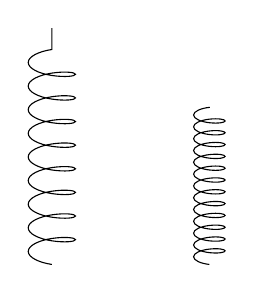
\begin{tikzpicture}
\draw[decoration={aspect=0.3, segment length=3mm, amplitude=3mm,coil},decorate] (0,0) -- +(0,3); 
\draw[decoration={aspect=0.3, segment length=1.5mm, amplitude=2mm,coil},decorate] (2,0) -- +(0,2); 
\end{tikzpicture}
\caption{Coils}
\end{marginfigure}

Verificando ainda a distensão da mola, podemos relacionar uma maior distensão a uma carga maior na caixa, isto é, quanto maior a força peso dos objetos pendurados na mola, maior a distensão. Experimentalmente, verifica-se que a relação entre o peso aplicado à mola e sua distensão são \emph{diretamente proporcionais}:
\begin{equation}
	\Delta x \propto P.
\end{equation}
%
Podemos então escrever para a \textbf{força elástica} $F_e$
\begin{equation}
	\vec{F}_e \propto -\vec{d},
\end{equation}
%
onde $\vec{d}$ representa o deslocamento $\Delta \vec{r}$ sofrido pela mola em módulo e direção, porém com a restrição que o deslocamento ocorra na direção longitudinal da mola. Podemos escrever a relação acima como uma igualdade introduzindo uma constante de proporcionalidade $k$:
\begin{equation}
	\vec{F}_e = -k \vec{d}.
\end{equation}

O resultado acima é conhecido como \emph{Lei de Hooke}, em homenagem ao físico inglês Robert Hooke, que o enunciou em 1660. Tal relação, no entanto, só é válida para pequenas distensões da mola. As distensões dentro deste limite são denominadas \emph{elásticas} e não deformam a mola permanentemente, caso contrário ao das distensões \emph{plásticas}. Apesar de a validade da Lei de Hooke ser limitada, ela é o modelo mais comum ao se analisar a resposta de um meio a uma deformação e pode ser utilizada como uma primeira aproximação mesmo para casos mais complexos.

%%%%%%%%%%%%%%%%%%%%%%%%%%%%%%%%%%%%%%
\section{Forças no movimento circular}
%%%%%%%%%%%%%%%%%%%%%%%%%%%%%%%%%%%%%%

De acordo com Newton:
\begin{quote}
    Uma força centrípeta é aquela pela qual corpos são puxados ou impelidos, ou tendem de alguma maneira, em direção a um ponto como um centro.
\end{quote}

Quando analisamos o movimento circular, verificamos que para o caso não uniforme -- o mais geral -- podemos dividir a aceleração em duas componentes com papeis distintos: a aceleração tangencial, responsável por alterar o módulo da velocidade, e a componente centrípeta, responsável por alterar a direção da velocidade. Como vimos, no entanto, para que haja uma aceleração, é necessário que haja uma força. 

Analisando um movimento unidimensional, temos que um objeto que se move em linha reta com certa velocidade precisa sofrer a atuação de uma força resultante para sofrer uma mudança no módulo de sua velocidade. Para um corpo que realiza um movimento circular, analogamente, se sua velocidade sofre uma mudança de direção -- mantendo constante seu módulo $\vec{v}$ --, o corpo também deve estar sujeito a atuação de uma força. No primeiro caso, a direção da força é a mesma do movimento (caso contrário o corpo sofreria uma alteração também da direção de seu movimento). No segundo caso, a força precisa atuar perpendicularmente à direção da velocidade (caso contrário sofreria uma alteração no módulo da velocidade). Da mesma forma que diferenciamos o papel exercido pelas acelerações tangencial e centrípeta, podemos diferenciar o papel entre uma força que aponta tangencialmente à trajetória e uma que aponta para o centro da trajetória circular: a primeira causa aceleração tangencial, alterando então o módulo da velocidade, já a segunda causa aceleração centrípeta, alterando então a direção do movimento. Denominamos a resultante de forças em direção ao centro da trajetória como \emph{Força centrípeta}. Podemos ter o resultado combinado dessas duas alterações (módulo e direção) quando exercemos uma força que faz um ângulo diferente de \degree{0} ou \degree{90} com a direção da velocidade.

Podemos utilizar a segunda lei de Newton e a expressão para a aceleração centrípeta
\begin{align}
  F &= ma \\
  a_c &= \frac{v^2}{R}
\end{align}
%
para relacionar a força exercida para manter um objeto em uma trajetória circular aos valores de massa, velocidade e raio da trajetória:
\begin{equation}
  F_c = m \frac{v^2}{R}. \mathnote{Força centrípeta.}
\end{equation}
%
Note, no entanto, que essa relação não nos diz nada sobre a natureza da força, ela simplesmente nos diz qual é a intensidade de força necessária para manter um objeto de massa $m$ em uma trajetória circular de raio $R$, com velocidade $v$. Se temos um corpo que gira preso a um fio, a força é uma tensão; Se temos um satélite em órbita em torno da Terra, temos a força gravitacional; Se temos um carro que faz uma curva em uma estrada plana, temos uma força de atrito. Em algumas situações, temos mais que uma força atuando de uma maneira complexa para manter um corpo em trajetória circular. Em um ``loop'' (uma curva vertical em uma pista), temos a atuação da força peso e da normal, porém em cada ponto da trajetória essas forças atuam de maneira diferente -- no topo ambas apontam para o centro da trajetória. Na parte inferior, a normal aponta para o centro e o peso para fora (sentido oposto ao centro) --. Em uma estrada com uma curva inclinada, temos uma \emph{componente} da normal e uma \emph{componente} da força de atrito. Note que a força centrípeta não é uma força nova, ela é uma \emph{força resultante que aponta para o centro da trajetória circular}.

Para facilitar a análise desse tipo de movimento, podemos tomar um eixo coordenado que ligue o corpo ao centro da trajetória circular, com sentido apontando para o centro da trajetória. Feito isso, basta tomar todas as componentes de força em tal direção, somá-las (levando em conta o sinal adequado) e igualá-las a $m v^4/R$. Veja a Figura ??? 
\comment{mega figura fullwidth (com equações) com uns três exemplos complicados com diagramas de força e o cálculo da força resultante que aponta no sentido do eixo radial, igualando-a depois a m $v^2/R$}

%%%%%%%%%%%%%%%%%%
\section{Aplicações} % na minha nova ideia, seria basicamente o que as aulas de dinâmica seriam
%%%%%%%%%%%%%%%%%%

\subsection{Leitura de uma balança em um elevador} 
Balança de subir (normal) e de pendurar (tensão).

\subsection{Blocos em contato}

\subsection{Bloco em plano inclinado}
Sem atrito, com atrito. Determinar $\mu_e$

\subsection{Blocos ligados por cordas}
Mostrar que podemos tratar tudo como um sistema unidimensional com um eixo x curvo

\subsection{Sistemas de roldanas}
Blá blá blá.

\subsection{Governador centrífugo} %ver wikipedia, tb é usado em geradores de eletricidade a gasolina

\subsection{Looping the loop}
Condição de perder contato e velocidade mínima

\subsection{Pendulo cônico}

\subsection{Curva compensada}

%%%%%%%%%%%%%%%%%%%%%%%%%%
\section{Seções opcionais}
%%%%%%%%%%%%%%%%%%%%%%%%%%

%%%%%%%%%%%%%%%%%%%%%%%%%%%%%%%%%%%%%
\subsection{Sistemas de massa variável}
%%%%%%%%%%%%%%%%%%%%%%%%%%%%%%%%%%%%%
%%%%%%%%%%%%%%%%%%%%%%%%%%%%%%%%%%%%%%%%%%%%%%
\subsection{Justificativa para a Lei de Hooke}
%%%%%%%%%%%%%%%%%%%%%%%%%%%%%%%%%%%%%%%%%%%%%%

A origem da força exercida por uma mola é a interação eletromagnética entre os átomos que a compõe. Essas forças eletromagnéticas não são lineares, porém, como temos uma quantidade muito grande de átomos, o deslocamento entre dois átomos ``vizinhos'' é muito pequeno. Nesse caso, a força apresenta um caráter aproximadamente linear. Isso pode ser entendido se levarmos em conta que qualquer função pode ser escrita como uma \emph{Série de Taylor}, isto é, como uma soma de suas derivadas:
\begin{equation}
	g(x) = g(a) + g'(a)(x - a) + g''(a)(x-a)^2 + g'''(a)(x-a)^3 + \dots,
\end{equation}
onde $g'(a)$, $g''(a)$, $g'''(a)$, etc. são as derivadas da função $g(x)$ calculadas no ponto $a$.

Utilizando esse resultado, podemos expandir uma função $f(x)$ qualquer que representa uma força unidimensional exercida em uma deformação. Escolhendo $a=0$, considerando que esta é a posição de equilíbrio, obtemos
\begin{equation}
	f(x) = f(0) + f'(0) (x-0) + f''(0)(x-0)^2 + \dots.
\end{equation}
%
No entanto, $f(0)$ é a força na posição de equilíbrio, ou seja, é zero -- caso contrário não seria um ponto de equilíbrio --. Além disso, se $x$ é muito pequeno, temos que $x^2$ é menor ainda e por isso podemos desprezar todos os termos de ordem 2 (termos quadráticos) ou maior. Obtemos então:
\begin{equation}
	f(x) = f'(0)x,
\end{equation}
%
e se fizermos $k \equiv f'(0)$,
\begin{equation}
	f(x) = kx.
\end{equation}
%
Essa relação é a própria lei de Hooke, porém para o caso unidimensional, com $x_i = 0$ e $x_f = x$. Além disso, falta o sinal que indica que a força é no sentido contrário ao deslocamento. A partir da análise acima, concluímos que quando falamos em pequenos deslocamentos, estamos restringindo os valores de termos de ordens quadrática ou superiores a valores muito menores que o termo de ordem linear. Respeitada essa condição, o que poder ser feito através da escolha de uma distensão máxima adequada, podemos tratar \emph{qualquer} deformação de um objeto como sendo linear.

%%%%%%%%%%%%%%%%%%%%%%%%%%%%%%%%%%%%%%%%%%%%%%%%%%%%%%%%%%%%
\subsection{Segunda lei do movimento de acordo com o Principia}
%%%%%%%%%%%%%%%%%%%%%%%%%%%%%%%%%%%%%%%%%%%%%%%%%%%%%%%%%%%%

\comment{TODO No parágrafo abaixo, fazer um footnote dizendo que não se justifica uma lei física, pois não há como fazer isso, isto é, uma lei fundamental é enunciada, não deduzida de algum outro lugar. (verificar se no The Character of the Physical Law do Feynmann tem alguma coisa do gênero). Como diz o M. Fiolhais, "tem-se que dar uma injeção".}
No \emph{Principia}, Newton não utiliza a discussão realizada acima para chegar à segunda lei. Após a definição de massa, ele apresenta a definição de \emph{movimento}, ou \emph{quantidade de movimento}, que atualmente denominamos como momento linear
\begin{quote}
\emph{A quantidade de movimento é a medida do mesmo, advindo da velocidade e da quantidade de matéria conjuntamente.}

O movimento do todo é a soma dos movimentos de todas as partes; e -- portanto -- em um corpo [com] o dobro em quantidade [de massa], com velocidade igual, o movimento é o dobro; com duas vezes a velocidade, é o quádruplo.
\end{quote}

Tendo em mente tais definições, Newton declara sua segunda lei do movimento como
\begin{quote}
\emph{A alteração do movimento é sempre proporcional à força motriz a ele aplicada; e é feita na direção da linha reta em que tal força atua.}

Se uma força qualquer gera um movimento, o dobro de força gerará o dobro de movimento, o triplo de força gera o triplo de movimento, seja a força aplicada subitamente, ou gradualmente. E este movimento (sendo sempre direcionado no mesmo sentido que a força geradora), se o corpo se encontrava em movimento, é adicionado a ele ou subtraído do movimento anterior, de acordo com eles conspirarem diretamente ou diretamente contrário um ao outro; ou composto obliquamente, quando são oblíquos, de tal forma a produzir um novo movimento composto pela determinação de ambos.
\end{quote}
%
Matematicamente, podemos escrever
\begin{equation}
  \Delta p \propto F.
\end{equation}
%
É claro também que $\Delta p \propto \Delta t$. Logo, se assumirmos que somente essas duas variáveis tem influência sobre a alteração do momento linear e considerando que a constante de proporcionalidade seja 1 (podemos engloba-la na própria definição da unidade de força), temos
\begin{equation}
  \Delta p = F \Delta t.
\end{equation}
%
Tomando o limite $\Delta t \to 0$, podemos escrever
\begin{equation}
  F = \frac{dp}{dt},
\end{equation}
%
ou, considerando $m$ como constante
\begin{align}
  F &= m\frac{dv}{dt} \\
  &= ma.
\end{align}

%%%%%%%%%%%%%%%%%%%%%%%%%%%%%%%%%%%%%%%%%%%%%%%%%%%%%%%%%%
\subsection{Equivalência das massas gravitacional e inercial}
%%%%%%%%%%%%%%%%%%%%%%%%%%%%%%%%%%%%%%%%%%%%%%%%%%%%%%%%%%

Veja que o fato de a aceleração gravitacional independer da massa se deve ao fato de que ela aparece em ambos os lados da igualdade na Equação~\eqref{Eq:EliminaM} acima. No entanto, isso se deve diretamente ao fato de que a força gravitacional depende da massa do corpo. Podemos citar um exemplo para deixar isso mais claro: a força entre duas cargas elétricas é dada por
\begin{equation}
  F_c = k \frac{q_1q_2}{r^2},
\end{equation}
%
uma expressão que segue a mesma forma da Lei da Gravitação, conhecida como Lei de Coulomb. Se uma partícula de massa $m$ e carga $q_p$ é atraída por uma esfera com carga $q_e$, temos pela segunda lei de Newton
\begin{equation}
  ma = \left[k \frac{q_e}{r^2}\right] q_p
\end{equation}
%
ou seja
\begin{equation}
  a = \left[k \frac{q_e}{r^2}\right] \frac{q_p}{m}.
\end{equation}
%
Isto é, existe uma dependência da aceleração com a massa da partícula.

A independência da aceleração gravitacional com a massa do corpo se deve ao fato de que a \emph{massa inercial} -- isto é, aquela que aparece na segunda lei de Newton -- é igual à \emph{massa gravitacional}. Isso não tem uma fundamentação teórica dentro da mecânica clássica pois ambos os fenômenos (a aceleração de um objeto submetido a uma força e a força entre tal objeto e a Terra) não têm nenhuma relação um com o outro. Para Newton, esta é uma verdade verificada experimentalmente.

\comment{Falar da interpretação do Einstein, da questão do elevador}

Voltando à expressão para a força gravitacional, vemos que a intensidade da força que atrai um objeto qualquer em direção à Terra é dada por
\begin{equation}
  F_g = m \left[G \frac{m_T}{r^2}\right],
\end{equation}
%
ou, se $r \approx r_T$
\begin{align}
  F_g &= mg \\
  &\equiv P,
\end{align}
%
isto é, a força peso nada mais é do que a força de atração gravitacional que atua sobre o corpo quando ele se encontra próximo da superfície da Terra. Notamos ainda que se o peso é o resultado da interação do corpo com a Terra, \emph{a reação à força peso é uma força que atua na Terra} -- ou, de maneira simplificada, no centro de massa da Terra --. Portanto, quando um objeto cai, sendo submetido a uma aceleração devida à força peso, temos que a reação ao peso atua na Terra, acelerando-a em direção ao objeto. Como vimos, no entanto, a aceleração é inversamente proporcional à massa e, devido ao fato de que a massa da Terra é muito grande, temos uma aceleração muito pequena por parte do Planeta.
\begin{marginfigure}[-5cm]
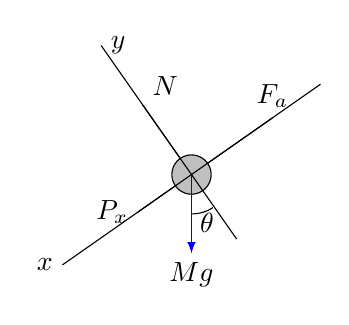
\begin{tikzpicture}[
    force/.style={>=latex,draw=blue,fill=blue},
    axis/.style={densely dashed,gray,font=\small},
    M/.style={circle,draw,fill=lightgray,minimum size=0.5cm,thin},
    m/.style={rectangle,draw=black,fill=lightgray,minimum size=0.3cm,thin},
    plane/.style={draw=black,fill=blue!10},
    string/.style={draw=red, thick},
    pulley/.style={thick},
	]
\def\iangle{35} % Angle of the inclined plane

\def\down{-90}
\def\arcr{0.5cm} % Radius of the arc used to indicate angles
 

    %% Free body diagram of M
    \begin{scope}[rotate=\iangle]
        \node[M,transform shape] (M) {};
        % Draw axes and help lines

        {[axis,->]
            \draw (0,-1) -- (0,2) node[right] {$y$};
            \draw (-2,0) node[left] {$x$} -- ++(4,0);
            % Indicate angle. The code is a bit awkward.

            \draw[solid,shorten >=0.5pt] (\down-\iangle:\arcr)
                arc(\down-\iangle:\down:\arcr);
            \node at (\down-0.5*\iangle:1.3*\arcr) {$\theta$};
        }

        % Forces
        {[force,->]
            % Assuming that Mg = 1. The normal force will therefore be cos(alpha)
            \draw (M.north) -- ++(0,{cos(\iangle)}) node[above right] {$N$};
            \draw (M.west) -- ++(-{sin(\iangle)},0) node[left] {$P_x$};
            \draw (M.east) -- ++(1,0) node[above] {$F_a$};
        }

    \end{scope}
    % Draw gravity force. The code is put outside the rotated
    % scope for simplicity. No need to do any angle calculations. 
    \draw[force,->] (M.center) -- ++(0,-1) node[below] {$Mg$};
    %%
\end{tikzpicture}
\caption{Teste Tikz.}
\end{marginfigure}

%%%%%%%%%%%%%%%%%%
\section{Apêndice}
%%%%%%%%%%%%%%%%%%

%%%%%%%%%%%%%%%%%%%%
\subsection{Diálogo}
%%%%%%%%%%%%%%%%%%%%

Segue abaixo uma tradução do trecho do \emph{Diálogo sobre os dois máximos sistemas do mundo: ptolomaico e copernicano} de Galileu Galilei, onde encontramos a discussão acerca do movimento contínuo e uniforme que ocorreria caso tivéssemos uma superfície horizontal de onde retirássemos todos os ``impedimentos ao movimento''.
% Dialogo, p. 83
\begin{description}
%\item[Salviati:]  Io non desidero che voi diciate o rispondiate di saper niente altro che quello che voi
%sicuramente sapete. Però ditemi: quando voi aveste una superficie piana, pulitissima come uno
%specchio e di materia dura come l'acciaio, e che fusse non parallela all'orizonte, ma alquanto
%inclinata, e che sopra di essa voi poneste una palla perfettamente sferica e di materia grave e
%durissima, come, verbigrazia, di bronzo, lasciata in sua libertà che credete voi che ella facesse? non
%credete voi (sí come credo io) che ella stesse ferma?
\item[Salviati:] [\dots] diga-me: quando você tem uma superfície plana, polidíssima com um espelho e de matéria dura como o aço, e que seja não paralela ao horizonte, mas um pouco inclinada, e que sobre ela você colocasse uma bola perfeitamente esférica e de material \emph{grave}\footnote{Um corpo \emph{grave} para Galileu é aquele que está sujeito à gravidade, ou seja, que se dirige ao centro da Terra quando pode se mover livremente.} e duríssima, como, por exemplo, de bronze, deixada em sua liberdade[,] o que você acredita que  ela faria? você não acredita (assim como creio eu) que ela continuaria parada?

%\item[Simplicio:]  Se quella superficie fusse inclinata?
\item[Simplicio:] Se aquela superfície fosse inclinada?

%\item[Salviati:]  Sí, ché cosí già ho supposto.
\item[Salviati:] Sim, é assim que supomos.

%\item[Simplicio:]  Io non credo che ella si fermasse altrimente, anzi pur son sicuro ch'ella si moverebbe
%verso il declive spontaneamente.
\item[Simplicio:] Eu não acredito que ela permaneça parada, antes estou seguro que ela se moverá para o declive espontaneamente.

%\item[Salviati:]  Avvertite bene a quel che voi dite, signor Simplicio, perché io son sicuro ch'ella si
%fermerebbe in qualunque luogo voi la posaste.
\item[Salviati:] Pense bem no que você disse, senhor Simplicio, por que eu estou seguro que ela ficará em qualquer lugar que você a colocar.

%\item[Simplicio:]  Come voi, signor Salviati, vi servite di questa sorte di supposizioni, io comincierò a non
%mi maravigliar che voi concludiate conclusioni falsissime.
\item[Simplicio:] Como você, senhor Salviati, se serve desse tipo de suposição, não me impressiona que você chegue a conclusões falsas.

%\item[Salviati:]  Avete dunque per sicurissimo ch'ella si moverebbe verso il declive spontaneamente?
\item[Salviati:] Você tem então por seguro que ela se moverá para o declive espontaneamente?

%\item[Simplicio:]  Che dubbio?
\item[Simplicio:] Que dúvidas?

%\item[Salviati:]  E questo lo tenete per fermo, non perché io ve l'abbia insegnato (perché io cercavo di
%persuadervi il contrario), ma per voi stesso e per il vostro giudizio naturale.
\item[Salviati:] E você tem isso por firme, não por que eu o tenha ensinado (por que eu tentava o persuadir do contrário), mas por você somente e pelo seu juízo natural.

%\item[Simplicio:]  Ora intendo il vostro artifizio: voi dicevi cosí per tentarmi e (come si dice dal vulgo) per
%iscalzarmi, ma non che in quella guisa credeste veramente.
\item[Simplicio:] Ora[,] entendo o seu artifício: você diz assim para me tentar e (como diz o povo) me desgastar, mas não que acredite verdadeiramente que seja assim. 

%\item[Salviati:]  Cosí sta. E quanto durerebbe a muoversi quella palla, e con che velocità? E avvertite che
%io ho nominata una palla perfettissimamente rotonda ed un piano esquisitamente pulito, per
%rimuover tutti gli impedimenti esterni ed accidentarii: e cosí voglio che voi astragghiate
%dall'impedimento dell'aria, mediante la sua resistenza all'essere aperta, e tutti gli altri ostacoli
%accidentarii, se altri ve ne potessero essere.
\item[Salviati:] De fato. E quanto duraria o movimento daquela bola, e com que velocidade? E perceba que eu supus uma bola perfeitissimamente redonda e um plano requintadamente polido, para remover todos os impedimentos externos e acidentais: e assim eu desejo que você [abstraia] o impedimento do ar, mediante à sua resistência em ser aberto, e todos os outros obstáculos acidentais, se outros puderem haver.

%\item[Simplicio:]  Ho compreso il tutto benissimo: e quanto alla vostra domanda, rispondo che ella
%continuerebbe a muoversi in infinito, se tanto durasse la inclinazione del piano, e con movimento
%accelerato continuamente; ché tale è la natura de i mobili gravi, che vires acquirant eundo: e quanto
%maggior fusse la declività, maggior sarebbe la velocità.
\item[Simplicio:] Compreendi tudo muito bem: e quanto à sua pergunta, respondo que ela continuará se movendo infinitamente, se tanto durasse a inclinação do plano, e com movimento acelerado continuamente; pois tal é a natureda dos corpos graves, que ``vai ganhar força'': e quanto maior for o declive, maior será a velocidade.

%\item[Salviati:]  Ma quand'altri volesse che quella palla si movesse all'insú sopra quella medesima
%superficie, credete voi che ella vi andasse?
\item[Salviati:] Mas quando outros desejassem que aquela bola se movesse para cima sobre aquela mesma superfície, você acredita que ela o faria?

%\item[Simplicio:]  Spontaneamente no, ma ben strascinatavi o con violenza gettatavi.
\item[Simplicio:] Espontaneamente não, mas arrastada ou jogada violentamente.

%\item[Salviati:]  E quando da qualche impeto violentemente impressole ella fusse spinta, quale e quanto
%sarebbe il suo moto?
\item[Salviati:] E quando de qualquer ímpeto violentamente impresso ela fosse impulsionada, qual e quanto seria seu movimento?

%\item[Simplicio:]  Il moto andrebbe sempre languendo e ritardandosi, per esser contro a natura, e sarebbe piú
%lungo o piú breve secondo il maggiore o minore impulso e secondo la maggiore o minore acclività.
\item[Simplicio:] O movimento seguiria sempre se abatendo e se retardando, pois ser contra a natureza, e será mais longo ou mais curto segundo o maior ou menor impulso e segundo maior ou menor for o aclive.

%\item[Salviati:]  Parmi dunque sin qui che voi mi abbiate esplicati gli accidenti d'un mobile sopra due
%diversi piani; e che nel piano inclinato il mobile grave spontaneamente descende e va continuamente
%accelerandosi, e che a ritenervelo in quiete bisogna usarvi forza; ma sul piano ascendente ci vuol
%forza a spignervelo ed anco a fermarvelo, e che 'l moto impressogli va continuamente scemando, sí
%che finalmente si annichila. Dite ancora di piú che nell'un caso e nell'altro nasce diversità dall'esser
%la declività o acclività del piano, maggiore o minore; sí che alla maggiore inclinazione segue
%maggior velocità, e, per l'opposito, sopra 'l piano acclive il medesimo mobile cacciato dalla
%medesima forza in maggior distanza si muove quanto l'elevazione è minore. Ora ditemi quel che
%accaderebbe del medesimo mobile sopra una superficie che non fusse né acclive né declive.
\item[Salviati:] Para mim até agora você me explicou os acidentes de um corpo que se movimenta sobre dois planos diferentes; e que no plano inclinado o corpo grave desce espontaneamente e vai continuamente acelerando-se, e que para o reter em repouso é necessário usar força; mas sobre o plano ascendente é necessário força para impulsioná-lo e também para o reter, e que o movimento impresso vai continuamente diminuindo, até que finalmente se aniquila. Ainda diz agora que num caso e no outro há diferença devida ao aclive ou declive do plano, [quanto a] ser maior ou menor; que à maior inclinação segue maior velocidade, e, pelo contrário, sobre o plano em aclive o mesmo corpo [sujeito] à mesma força se move em distância tanto maior quanto menor é a elevação. Ora[,] diga-me o que aconteceria com o mesmo corpo sobre uma superfície que não é nem em aclive[,] nem em declive?

%\item[Simplicio:]  Qui bisogna ch'io pensi un poco alla risposta. Non vi essendo declività, non vi può essere
%inclinazione naturale al moto, e non vi essendo acclività, non vi può esser resistenza all'esser mosso,
%talché verrebbe ad essere indifferente tra la propensione e la resistenza al moto: parmi dunque che e'
%dovrebbe restarvi naturalmente fermo. Ma io sono smemorato, perché non è molto che 'l signor
%Sagredo mi fece intender che cosí seguirebbe.
\item[Simplicio:] Aqui é necessário que eu pense um pouco sobre a resposta. Não havendo declividade, não pode haver inclinação natural ao movimento, e não havendo aclive, não pode existir resistência ao movimento, tal que se faria indiferente entre à propensão e à resistência ao movimento: para mim então o que deve acontecer é permanecer naturalmente parado. [...]

%\item[Salviati:]  Cosí credo, quando altri ve lo posasse fermo; ma se gli fusse dato impeto verso qualche
%parte, che seguirebbe?
\item[Salviati:] Assim o creio, quando alguém o colocar parado: mas e se lhe fosse dado ímpeto para qualquer parte, o que aconteceria?

%\item[Simplicio:]  Seguirebbe il muoversi verso quella parte.
\item[Simplicio:] Seguiria se movendo em direção àquela parte.

%\item[Salviati:]  Ma di che sorte di movimento? di continuamente accelerato, come ne' piani declivi, o di
%successivamente ritardato, come negli acclivi?
\item[Salviati:] Mas que tipo de movimento? continuamente acelerado, como num plano em declive, ou sucessivamente retardado, como num aclive?

%\item[Simplicio:]  Io non ci so scorgere causa di accelerazione né di ritardamento, non vi essendo né
%declività né acclività.
\item[Simplicio:] Eu não decifro nenhuma causa de aceleração[,] nem de retardamento, não havendo aclive ou declive.

%\item[Salviati:]  Sì. Ma se non vi fusse causa di ritardamento, molto meno vi dovrebbe esser di quiete:
%quanto dunque vorreste voi che il mobile durasse a muoversi?
\item[Salviati:] Sim. Mas se não existisse causas para o retardamento, muito menos deveria estar em repouso: então quanto tempo você [acha] que o movimento do corpo deve durar?

%\item[Simplicio:]  Tanto quanto durasse la lunghezza di quella superficie né erta né china.
\item[Simplicio:] Tanto quanto durasse a extensão daquela superfície [...]

%\item[Salviati:]  Adunque se tale spazio fusse interminato, il moto in esso sarebbe parimente senza
termine, cioè perpetuo?
\item[Salviati:] Portanto se tal espaço fosse interminável, o movimento nele seria também sem fim, seria perpétuo?

%\item[Simplicio:]  Parmi di sí, quando il mobile fusse di materia da durare.
\item[Simplicio:] Para mim sim, quando o corpo for de material que durasse.

%\item[Salviati:]  Già questo si è supposto, mentre si è detto che si rimuovano tutti gl'impedimenti
%accidentarii ed esterni, e la fragilità del mobile, in questo fatto, è un degli impedimenti accidentarii.
%Ditemi ora: quale stimate voi la cagione del muoversi quella palla spontaneamente sul piano
%inclinato, e non, senza violenza, sopra l'elevato?
\item[Salviati:] Isso já é suposto, enquanto e é dido que se removem todos os impedimentos acidentais e esternos, e a fragilidade do corpo, e este fato é um dos impedimentos acidentais. Diga-me agora: qual você acha ser a razão  daquela bola se mover espontaneamente sobre o plano inclinado, e não, sem violência, sobre o elevado?

%\item[Simplicio:]  Perché l'inclinazion de' corpi gravi è di muoversi verso 'l centro della Terra, e solo per
%violenza in su verso la circonferenza; e la superficie inclinata è quella che acquista vicinità al centro,
%e l'acclive discostamento.
\item[Simplicio:] Por que a tendência dos corpos graves é de se mover para o centro da Terra, e somente por violência contra a circunferência [isto é, para cima]; e a superfície inclinada é aquela que dá proximidade com o centro, e o aclive distanciamento.

%\item[Salviati:]  Adunque una superficie che dovesse esser non declive e non acclive, bisognerebbe che in
%tutte le sue parti fusse egualmente distante dal centro. Ma di tali superficie ve n'è egli alcuna al
%mondo?
\item[Salviati:] Portanto uma superfície que devesse ser sem declive e sem aclive, necessita que todas as suas partes sejam igualmente distantes do centro. Mas tal superfície, há alguma no mundo?\footnote{A interpretação usual dessa afirmação é de que para Galileu o movimento ocorre naturalmente como um círculo sobre a superfície da Terra. No entanto, essa interpretação de inércia circular é contestada com base em outros trabalhos de Galileu. Vide referência abaixo.}\cite{Vasconcelos2005}

%\item[Simplicio:]  Non ve ne mancano: ècci quella del nostro globo terrestre, se però ella fusse ben pulita, e
%non, quale ella è, scabrosa e montuosa; ma vi è quella dell'acqua, mentre è placida e tranquilla.
\item[Simplicio:] [\dots] é aquela do nosso globo terrestre, se no entanto ela fosse bem polida, e não, qual ela é, escabrosa e montanhosa; mas como é aquela da água, enquanto está plácida e tranquíla.

%\item[Salviati:]  Adunque una nave che vadia movendosi per la bonaccia del mare, è un di quei mobili che
%scorrono per una di quelle superficie che non sono né declivi né acclivi, e però disposta, quando le
%fusser rimossi tutti gli ostacoli accidentarii ed esterni, a muoversi, con l'impulso concepito una
%volta, incessabilmente e uniformemente
\item[Salviati:] Portanto um navio que vai movendo-se pela calmaria do mar, é um dos corpos que escorrem por uma dessas superfícies que não são nem aclives nem declives, e assim disposta, quando lhe removermos todos os obstáculos acidentais e externos, a mover-se, com o impulso concebo um movimento, incessante e uniforme.

%\item[Simplicio:] Par che deva esser cosí.
\item[Simplicio:] É assim que deve ser.

\end{description}
